%%%%%%%%%%%%%%%%%%%%%%%%%%%%%%%%%%%%%%%%%%%%%%
%Lab report writeup based on template by Derek Hildreth
%%%%%%%%%%%%%%%%%%%%%%%%%%%%%%%%%%%%%%%%%%%%%%

%\documentclass[aps,letterpape,10pt]{revtex4}
\documentclass[aps,letterpaper,10pt]{article}
%\documentclass{article}

\usepackage{graphicx} % For images
\usepackage{float}    % For tables and other floats
\usepackage{verbatim} % For comments and other
\usepackage{amsmath}  % For math
\usepackage{amssymb}  % For more math
\usepackage{fullpage} % Set margins and place page numbers at bottom center
\usepackage{subfig}   % For subfigures
\usepackage[usenames,dvipsnames]{color} % For colors and names
\usepackage{fancyhdr} %headers
\usepackage{listings} %for code
\usepackage{color} %to color code
\usepackage{wrapfig} % for inline images

%Color and code setup
\definecolor{dkgreen}{rgb}{0,0.6,0}
\definecolor{gray}{rgb}{0.5,0.5,0.5}
\definecolor{mauve}{rgb}{0.58,0,0.82}
\definecolor{codebg}{rgb}{.95,.95,.98}

\lstset{ %
	language=Java,
	tabsize=4, 
	numbers=left,
	numberstyle=\footnotesize,
	backgroundcolor=\color{codebg},
	breaklines=true,
	breakatwhitespace=true,
	basicstyle=\small,
	numberstyle=\tiny\color{black},
	showstringspaces=false,
	keywordstyle=\color{blue}, 
	stringstyle=\color{dkgreen},
	commentstyle=\color{gray},
	frame=single,
	title = \texttt{\lstname}
	}

%%%%%%%%%%%%

%HEADER FORMATING%%%%%%%%%%%%%
\pagestyle{fancy}
\headheight 10pt
\setlength{\headsep}{20pt}
\lhead{PHYS 251 - Prof. Tom Witten \\ Project 2}
\rhead{A. Athanassiadis\\Due 10/26/2012}
%%%%%%%%%%%%%%%%%%%%%%%%

%Custom Definitions%%%%%%%%%%%%%%%
\newcommand{\ttt}{\texttt}
%%%%%%%%%%%%%%%%%%%%%%%%

\begin{document}

\section{Part 1}

I studied the two functions 
\begin{eqnarray*}
f_1(x) & = & r * x * (1-x) \\
f_1(x) & = & r * x * (1-x) * (2-x) * (3-x)
\end{eqnarray*}

Which both satisfy the following properties:
\begin{enumerate}
\item $f(0) = f(1) = 1$
\item $f''(x) < 0$
\item $f_x = r * f_0(x)$
\item $f: [0,1]\to [0,1]$
\end{enumerate}

Using my code in \ttt{LogisticMap2.java}, I generated the following two images:

\begin{figure}[!h]
\centering
\subfloat[Iterated results for $f_1(x;r)$]{\label{im:LogMap1}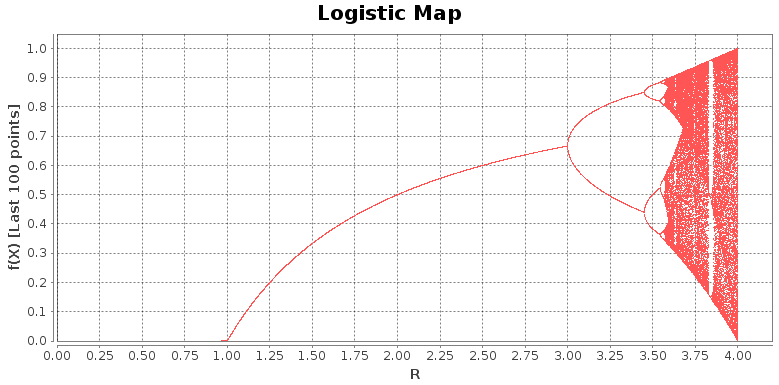
\includegraphics[width=.49\textwidth]{../pictures/LogMap1.png}}
\subfloat[Iterated results for $f_2(x;r)$]{\label{im:LogMap2}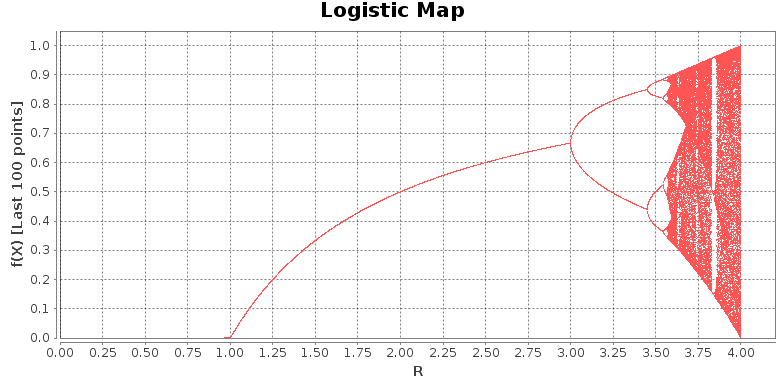
\includegraphics[width=.49\textwidth]{../pictures/LogMap2.png}}
\label{fig:LogMap}
\end{figure}

It is evident that there is very little different in the high-iteration appearance of the iterated maps $f_1$ and $f_2$. I produced these plots by iterating through r, and at each value of r, iterating f 1000 times. In order to clean up the output, I only returned the last 100 results of iteration using a buffer that was filled once the iteration counter passed 900. The rational behind this is that the early behavior of iteration are strongly related to the initial value of x (which was set randomly for me). However, due to the nature of the maps $f_i$ used, convergence to the fixed points (or cycles) was quick.


\section{Part 2}
For the map $f(x) = rx(1-x)$, we can analytically solve for the bifurcation points in r. \\

Begin with the hypothesis that there is an $r=r_2$ such that $f$ develops a 2-cycle. This corresponds to the onset of a stable fixed point of $f^{(2)}$, and the occurrence of an instability in $f$. From our derivations in class, the instability in $f$ corresponds to the point at which $f'(x^\star)=-1$. \\

Solving for $f(x^\star) = x^\star$ we find that $$(x^\star) = 1-\frac{1}{r}.$$

\newpage
Using this, we can solve for $r_2$:

\begin{eqnarray*}
-1 & = & f'(x^\star) \\
   & = & \frac{d}{dx}(rx(1-x))|_{x^\star} \\
   & = & r_2 (1-2x^\star) \\
   & = & r_2 (1-2(1-\frac{1}{r_2})) \\
   & = & -r_2 + 2
\end{eqnarray*}

Hence, $$r_2 = 3$$
and plugging back in, we see that at $r_2$, $$x^\star |_{r_2} = \frac{2}{3} = .666.$$

\section{Part 3}

Using the Newton-Raphson method, and $r$ values taken from the above plot of $f_1$, I numerically determined the fixed points of $f$ when it has stable 2 and 4 cycles. The guesses for the method were the result of iterating the function 10 times from a random start value. \\

\begin{center}
\begin{tabular}{|r|r|r|r|}
\hline
n-cycle & $r$ & guess $x_0$ & converged value $x^\star$ \\
\hline
2 & 3.2 & 0.513 & 0.513 \\
  &     & 0.799 & 0.798 \\
\hline
4 & 3.5 & 0.840 & 0.501 \\
  &     & 0.471 & 0.827 \\
  &     & 0.872 & 0.875 \\
  &     & 0.391 & 0.383 \\
\hline
\end{tabular}
\end{center}

As is evident by some of the above (guess,converged value) pairs, the iterations converge very quickly to the fixed points. The convergence tolerance for Newton-Raphson was $1e-9$. The delta used for derivatives was $1e-6$.

\section{Part 4}

In \ttt{Floquet.java}, I plot the Floquet Multiplier $\Lambda|_{f^{(N)}} = \frac{df^{(N)}}{dx}|_{x^\star}$ (L in code) against $r$. As expected, at each bifurcation of $f^{(N)}$, $\Lambda|_{f^{(2N)}}=-1$. See the figure below for $N=2,4,8$. As you can see, at each bifurcation, $f(N)$ splits into an equal number of stable and unstable fixed points.
\newpage

\begin{figure}[!h]
\centering
\subfloat[Floquet Multiplier of $f$ ]{\label{im:FloquetBig1}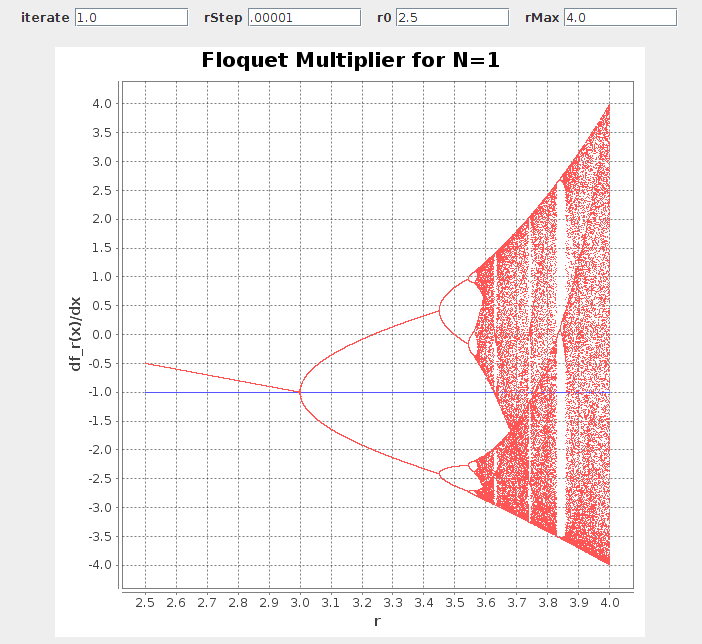
\includegraphics[width=.4\textwidth]{../pictures/floquet-full.png}} \hfill
\subfloat[Bifurcation of $f$ at $r_2$]{\label{im:Floquet2}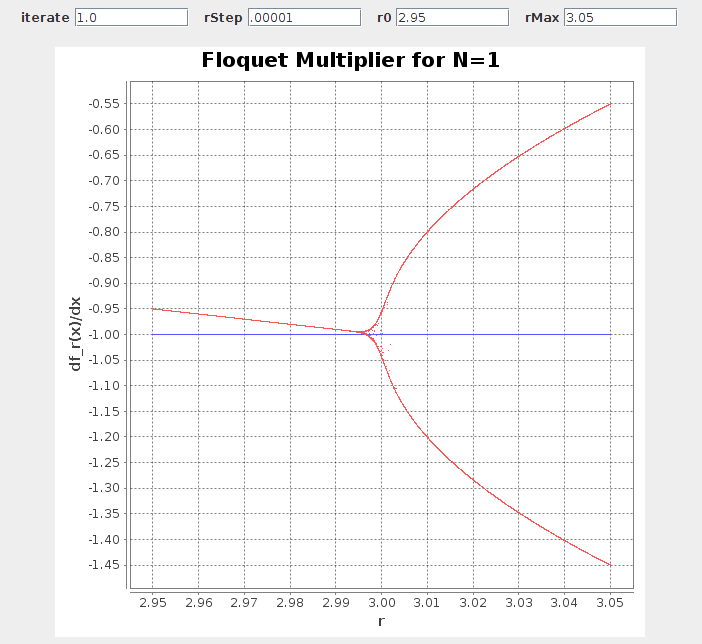
\includegraphics[width=.4\textwidth]{../pictures/floquet-zoom2.png}} \\
\subfloat[Double Bifurcation of $f^{(4)}$ at $r_4$]{\label{im:Floquet4}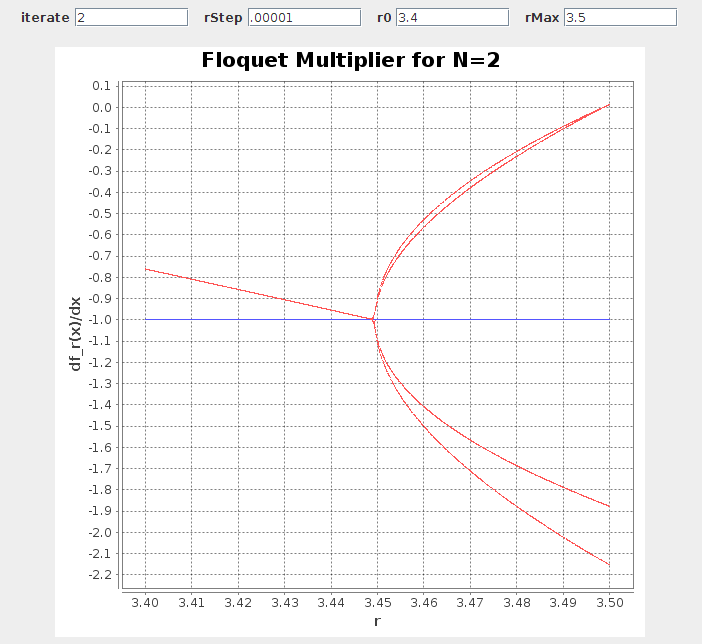
\includegraphics[width=.4\textwidth]{../pictures/floquet-zoom4-n2.png}} \hfill
\subfloat[Quad Bifurcation of $f^{(8)}$ at $r_8$]{\label{im:Floquet8}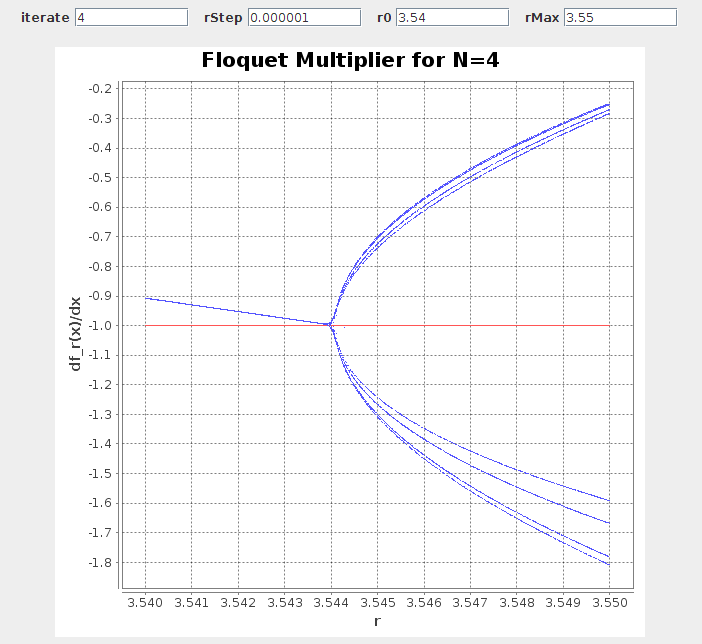
\includegraphics[width=.4\textwidth]{../pictures/floquet-zoom8-n4.png}}
\label{fig:Floquet}
\end{figure}

\newpage
\section{Part 5}

I looked at the behavior of $f$ at 4 values of $r$ where the logistic map curve exhibited interesting behavior. In each of the following subsections, there is a picture of the region around the interesting $r$ as well as a brief discussion of the occurrences there.\\

\subsection{$r\approx3.68$}
\begin{figure}[!h]
\centering
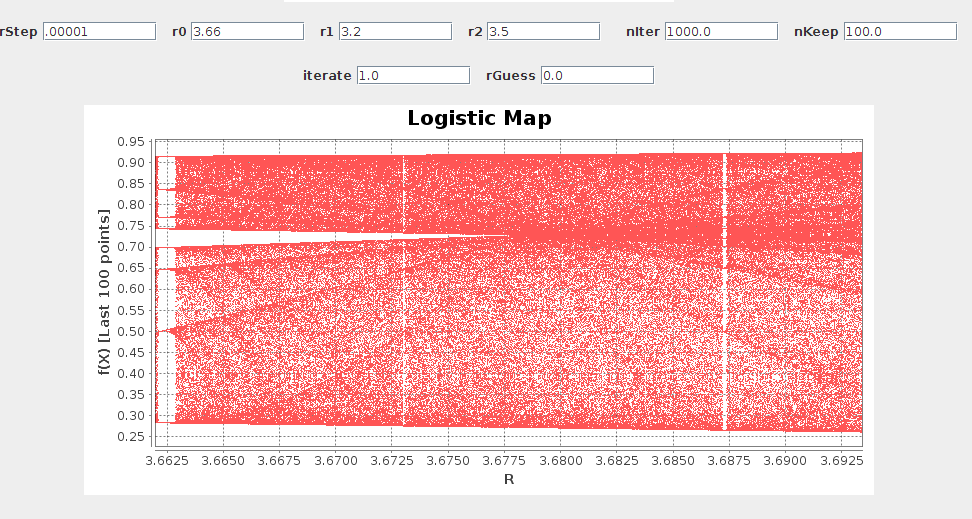
\includegraphics[width=\textwidth]{../pictures/CoolPic1.png}
\label{fig:r1}
\end{figure}

At this point, $r_\infty$, the function is involved in an infinite cycle. For smaller $r$, the cycles were finite in length, growing like $2^N$. Visually, two halves meet that had originally split from the instability as $N=1\to N=2$.

\subsection{$r\approx3.83$}
\begin{figure}[!h]
\centering
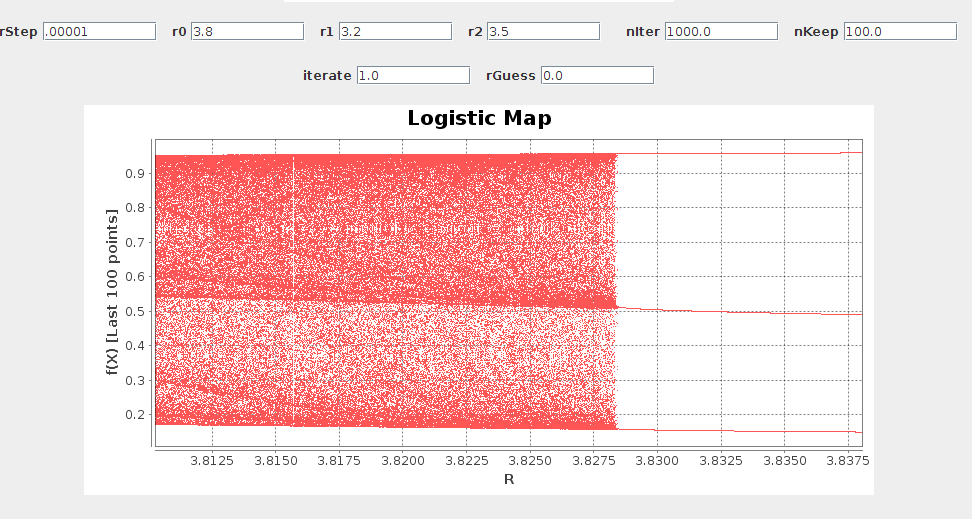
\includegraphics[width=\textwidth]{../pictures/CoolPic2.png}
\label{fig:r2}
\end{figure}
Here, the mess that had emerged after $r_\infty$ seems to have converged back into a stable 3-cycle. This is rather confusing at first glance. Why should something that went infinite spontaneously reemerge as finite. Moreover, what sets that transition value $r_{strange}$?

\newpage
\subsection{$r\approx3.8568$}
\begin{figure}[!h]
\centering
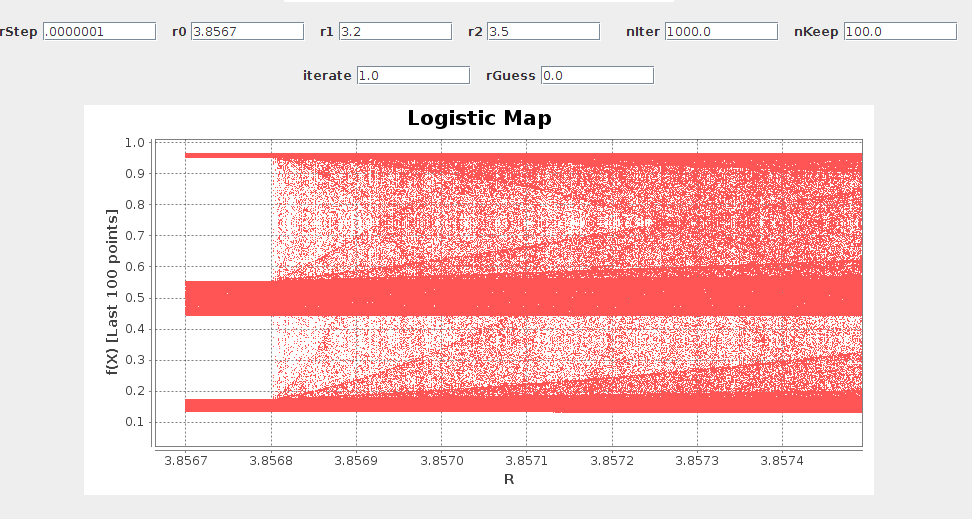
\includegraphics[width=\textwidth]{../pictures/CoolPic3.png}
\label{fig:r3}
\end{figure}

The stable 3 cycle found in the previous plot began to bifurcate repeatedly again. However, before the outermost bifurcation paths intersected again, a ``wall of cycles'' occurs again. Because of the resolution of my plot and the lack of any buildup, this feature seems to be one of the Logistic map and not an artifact of the numerics. Once again, this spontaneous phase transition is perplexing - what sets the $r_{crit}$ and what is the length of the cycle that it jumps to there?

\subsection{$r=4$}
\begin{figure}[!h]
\centering
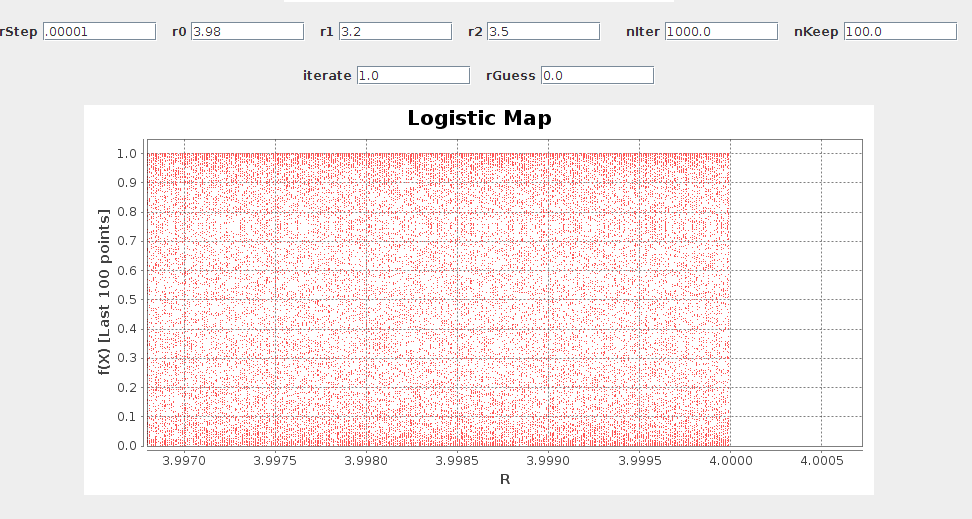
\includegraphics[width=\textwidth]{../pictures/CoolPic4.png}
\label{fig:r4}
\end{figure}

For our logistic map function, $r=4$ is the maximum allowed $r$ value. That being the case, it is also the only value of $r$ for which 1 is in the range of $f$. Naturally, this seems like a reasonable point to see some sort of new behavior, whether it is convergence or something else. However, upon inspection, the lefthand limit reveals no such interesting behavior. Hence I mark this as an interesting point because the features of the curve do not appear to change as $r\to4$ from the left, so there is either a discontinuity in the behavior of $f$ at $r=4$ or it is continuous and there is a seemingly ``normal'' behavior beyond what is allowed in our system.





\newpage
\lstinputlisting{../LogisticMap2.java}
\newpage
\lstinputlisting{../Floquet.java}

\end{document} 
